\documentclass[a4paper, 11pt]{report}

\usepackage{lmodern}
\usepackage[french]{babel}
\usepackage[utf8]{inputenc}
\usepackage[T1]{fontenc}

\usepackage{graphicx} % Pour les images
\graphicspath{Figures}
\usepackage{caption}
\usepackage{subcaption}
\usepackage{amsmath, amsfonts, amssymb} %Pour les maths

\usepackage{textcase}

\usepackage{afterpage}

% La numérotation

\makeatletter\@addtoreset{section}{chapter}\makeatother
\renewcommand{\thepart}{\Roman{part}}
\renewcommand{\thechapter}{\arabic{chapter}}
\renewcommand{\thesection}{\Roman{section}}

\usepackage{chngcntr}
\counterwithin{figure}{section}

% Sommaire + hyperliens
% \usepackage{bookmark}
\usepackage[hyphens]{url}
\usepackage[pdfauthor = {{Baptiste Braun-Delvoye, Julien Sagnes}}, pdftitle = {{Rapport de Projet}}, pdfstartview = Fit, pdfpagelayout = SinglePage, pdfnewwindow = true, bookmarksnumbered = true, breaklinks, colorlinks, linkcolor = black, urlcolor = black, citecolor = black, linktoc = all]{hyperref}
\usepackage[
    left = \flqq{},% 
    right = \frqq{},% 
    leftsub = \flq{},% 
    rightsub = \frq{} %
]{dirtytalk} % permet de citer mieux

% Codes

\usepackage{listings}
\usepackage{xcolor}
\usepackage[section]{placeins}
\usepackage{enumitem}
\usepackage{accsupp}

\newcommand{\noncopynumber}[1]{%
    \BeginAccSupp{method=escape,ActualText={}}%
    #1%
    \EndAccSupp{}%
}

\definecolor{codegreen}{rgb}{0,0.6,0}
\definecolor{codegray}{rgb}{0.5,0.5,0.5}
\definecolor{codepurple}{rgb}{0.58,0,0.82}
\definecolor{backcolour}{rgb}{0.95,0.95,0.92}

\lstdefinestyle{mystyle}{
    backgroundcolor=\color{backcolour},   
    commentstyle=\color{codegreen},
    keywordstyle=\color{magenta},
    numberstyle=\tiny\color{codegray},
    stringstyle=\color{codepurple},
    basicstyle=\ttfamily\footnotesize,
    breakatwhitespace=false,         
    breaklines=true,                 
    captionpos=b,                    
    keepspaces=true,                 
    numbers = left,
    numberstyle=\tiny\noncopynumber,
    numbersep=5pt,                  
    showspaces=false,                
    showstringspaces=false,
    showtabs=false,                  
    tabsize=2,
    literate=
  {á}{{\'a}}1 {é}{{\'e}}1 {í}{{\'i}}1 {ó}{{\'o}}1 {ú}{{\'u}}1
  {Á}{{\'A}}1 {É}{{\'E}}1 {Í}{{\'I}}1 {Ó}{{\'O}}1 {Ú}{{\'U}}1
  {à}{{\`a}}1 {è}{{\`e}}1 {ì}{{\`i}}1 {ò}{{\`o}}1 {ù}{{\`u}}1
  {À}{{\`A}}1 {È}{{\'E}}1 {Ì}{{\`I}}1 {Ò}{{\`O}}1 {Ù}{{\`U}}1
  {ä}{{\"a}}1 {ë}{{\"e}}1 {ï}{{\"i}}1 {ö}{{\"o}}1 {ü}{{\"u}}1
  {Ä}{{\"A}}1 {Ë}{{\"E}}1 {Ï}{{\"I}}1 {Ö}{{\"O}}1 {Ü}{{\"U}}1
  {â}{{\^a}}1 {ê}{{\^e}}1 {î}{{\^i}}1 {ô}{{\^o}}1 {û}{{\^u}}1
  {Â}{{\^A}}1 {Ê}{{\^E}}1 {Î}{{\^I}}1 {Ô}{{\^O}}1 {Û}{{\^U}}1
  {œ}{{\oe}}1 {Œ}{{\OE}}1 {æ}{{\ae}}1 {Æ}{{\AE}}1 {ß}{{\ss}}1
  {ű}{{\H{u}}}1 {Ű}{{\H{U}}}1 {ő}{{\H{o}}}1 {Ő}{{\H{O}}}1
  {ç}{{\c c}}1 {Ç}{{\c C}}1 {ø}{{\o}}1 {å}{{\r a}}1 {Å}{{\r A}}1
  {€}{{\EUR}}1 {£}{{\pounds}}1
}
\lstset{style=mystyle}
  
% Bibliographie

\usepackage{csquotes}
\usepackage[backend=biber,style=ieee,sorting=none]{biblatex}
\addbibresource{biblio.bib}

% \title{Rapport Stage Pantographe Haptique}
% \author{Baptiste Braun-Delvoye, Axel Gricourt}
% \date{October 2023}

\begin{document}

\definecolor{darkWhite}{rgb}{0.94,0.94,0.94}

% Page de garde

\begin{titlepage}
    \newcommand{\HRule}{\rule{\linewidth}{0.5mm}}
    \begin{center}
        \begin{minipage}{1\linewidth}
            \begin{flushleft}
                \hspace{4.5cm}
                
\includegraphics[width=0.25\textwidth]{Figures/SORBONNE_FAC_SCIENCES_DEF_CMJN.pdf}
            \end{flushleft}
        \end{minipage}

        \vspace{1.5cm}
        
        \textsc{\Large{}Master SAR 1\up{\MakeTextLowercase{ère}} année} \\[0.5cm]
        \textsc{\large{}2024 - 2025} \\[0.5cm]

        \HRule \\[0.6cm]
        {\huge\bfseries{}Rapport de Projet de Modélisation :} \\ \LARGE{Conception, Modélisation et Commande d'un robot parallèle 3RRR} \\[0.25cm]
        \HRule \\[1.5cm]


        \Large\textit{Auteurs :}\\
        \begin{center}
            Baptiste \textsc{Braun-Delvoye}\\
            Julien \textsc{Sagnes}
        \end{center}

        \hfill

        \Large\textit{Professeur :}\\
        \begin{center}
            Faiz \textsc{Ben-Amar}
        \end{center}
        \vspace{1cm}
        {\large\today} \\[2cm]
    \end{center}

    \vfill
\end{titlepage}


\selectlanguage{french} 
% \addcontentsline{toc}{section}{Abstract}

\clearpage\setcounter{page}{2}

\tableofcontents

\section*{Introduction}
\addcontentsline{toc}{section}{Introduction}

\section{Conception}

Pour la conception, nous utilisons le logiciel SolidWorks. Nous avons décidé de suivre le modèle du TP pour dessiner les différentes pièces, 
en s'assurant de garder des distances de l'ordre de la dizaine de centimètre ; nous nous assurons de ne pas concevoir un robot trop grand.

\subsection{Bras du robot}


\begin{figure}[h]
    \centering
    \begin{subfigure}[t]{0.50\textwidth}
        \centering
        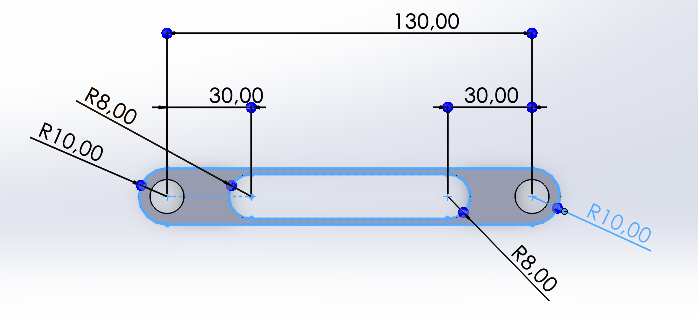
\includegraphics[width=\textwidth]{Figures/bras_effecteur.png}
        \caption{Bras effecteur}
    \end{subfigure}
    \hfill
    \begin{subfigure}[t]{0.45\textwidth}
        \centering
        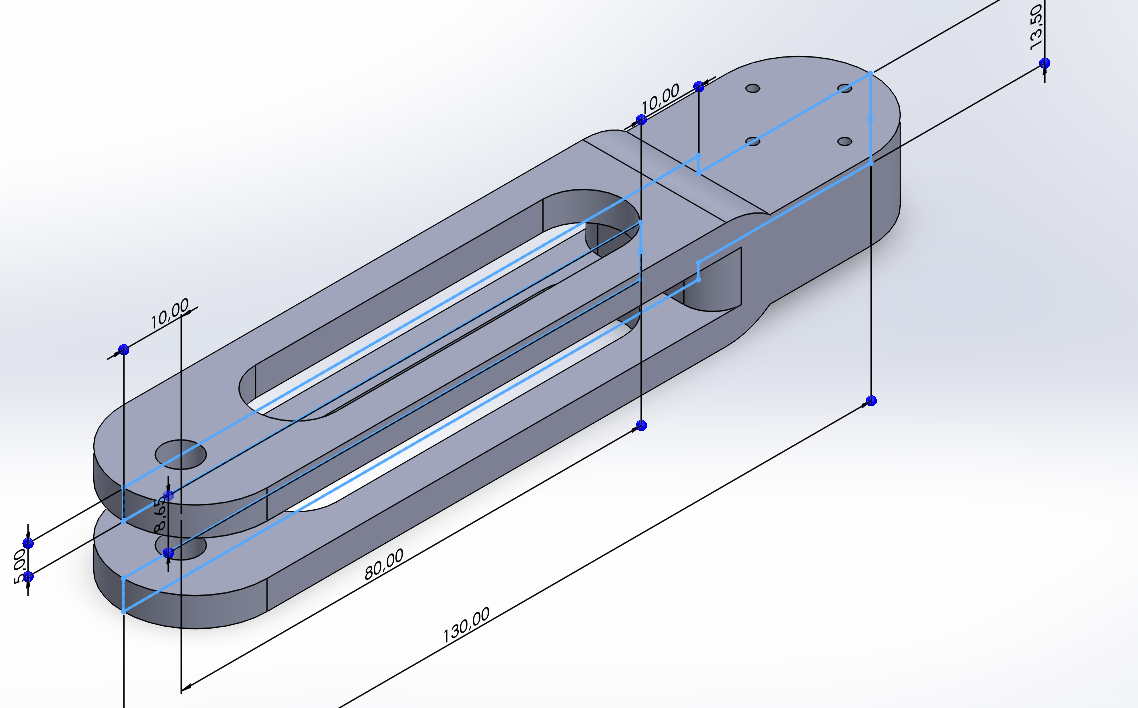
\includegraphics[width=\textwidth]{Figures/bras_moteur.png}
        \caption{Bras moteur}
    \end{subfigure}
    \caption{Allègement des bras du robot}
    \label{fig:bras}
\end{figure}

Dans un premier temps, nous concevons les bras qui composent le robot pour décider de la taille générale de la maquette.
Également, il est question de minimiser la quantité de matériaux utilisée pour les différentes pièces dans l'objectif de réduire le coût d'impression 3D.
Nous opérons donc une optimisation topologique sur les différents bras en effectuant des allègements, comme nous pouvons le voir sur la figure \ref{fig:bras}, 
qui détaille aussi les côtes des pièces en millimètres. Du reste, nous utilisons des congés pour adoucir les bords des pièces afin de rendre le robot plus harmonieux.

\subsection{Effecteur}


\begin{figure}[!tbh]
    \centering
    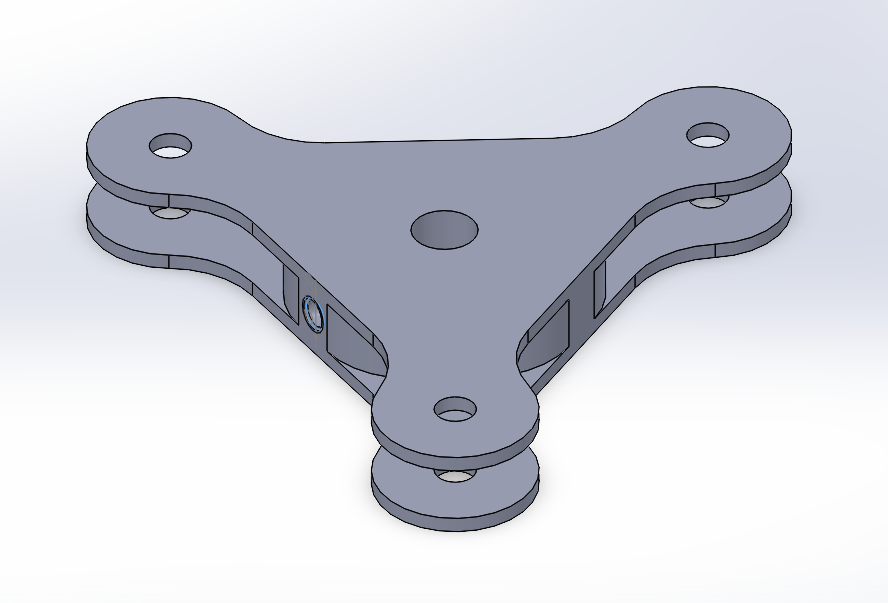
\includegraphics[width=0.5\textwidth]{Figures/effecteur.png}
    \caption{Effecteur}
    \label{fig:effecteur}
\end{figure}
Pour l'effecteur, nous optons pour une forme triangulaire, dont les côtés sont agencés de telle sorte qu'ils puissent auceuillir les boulons.
En effet, les trous que nous faisons sur les pièces (liaison pivot entre les bras et l'effecteur)
ont pour but d'acceuillir des boulons M6 (diamètre du trou 6.3 mm), auquel on rajoute un jeu de 0.15 mm.
Dans un but de maximisation de l'espace de travail, nous effectuons des extrusions sur le bord de la pièce pour éviter les blocages et assurer une rotation libre,
comme nous pouvons le voir sur la figure \ref{fig:effecteur}. 
Nous ajoutons également un trou au centre pour acceuillir un stylo que l'on serre avec une vis M5.

\subsection{Moteur}

% [\cite{hamdoun_inverse_2015}]

\begin{figure}[!tbh]
    \centering
    \begin{subfigure}[t]{0.45\textwidth}
        \centering
        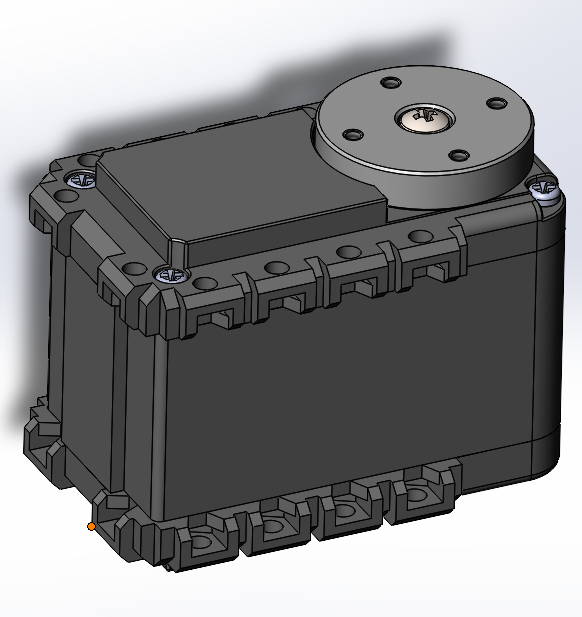
\includegraphics[width=\textwidth]{Figures/moteur_AX12.png}
        \caption{Moteur assemblé}
    \end{subfigure}
    \hfill
    \begin{subfigure}[t]{0.50\textwidth}
        \centering
        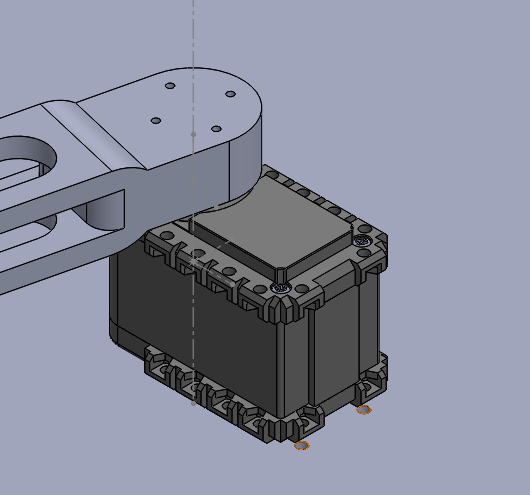
\includegraphics[width=\textwidth]{Figures/moteur_accroche.png}
        \caption{Moteur accroché}
    \end{subfigure}
    \caption{Moteur AX12}
    \label{fig:moteur}
\end{figure}
Quant aux moteurs, nous avons importé le cerveau moteur de type AX12 de Dynamixel que nous fixerons au bras grâce à quatre vis M2, comme nous pouvons le voir sur la figure \ref{fig:moteur}.

\subsection{Assemblage}

\begin{figure}[!tbh]
    \centering
    \begin{subfigure}[t]{0.48\textwidth}
        \centering
        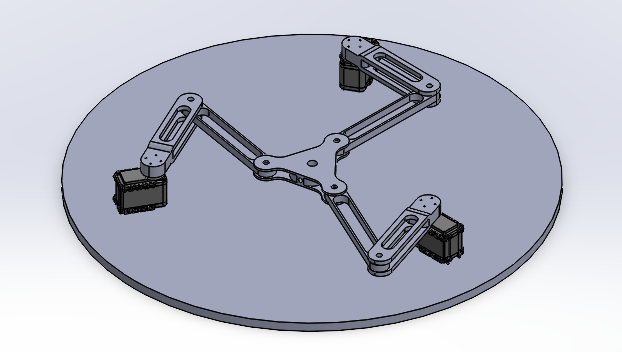
\includegraphics[width=\textwidth]{Figures/assemblage_1.png}
        \caption{Assemblage du robot}
    \end{subfigure}
    \hfill
    \begin{subfigure}[t]{0.48\textwidth}
        \centering
        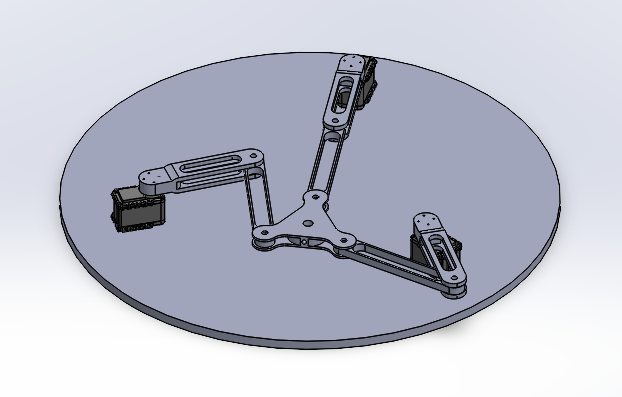
\includegraphics[width=\textwidth]{Figures/assemblage_2.png}
        \caption{Assemblage après mouvement}
    \end{subfigure}
    \caption{Assemblage sur SolidWorks}
    \label{fig:assemblage}
\end{figure}

Enfin, nous effectuons l'assemblage du robot en utilisant des contraintes standards de coaxialité et de coïncidence pour les vis, et des liaisons pivots entre les bras et l'effecteur. Nous accrochons ensuite les moteurs à une base fixe pour que ces derniers restent immobiles, comme illustré sur la figure \ref{fig:assemblage}.

\subsection{Singularités}

\begin{figure}[!tbh]
    \centering
    \begin{subfigure}[t]{0.48\textwidth}
        \centering
        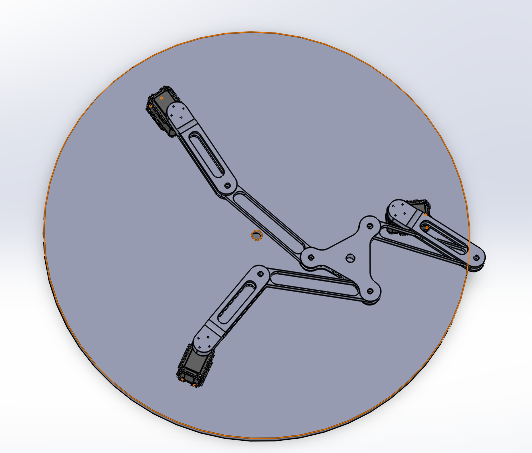
\includegraphics[width=\textwidth]{Figures/singularité série.png}
        \caption{Singularité série}
    \end{subfigure}
    \hfill
    \begin{subfigure}[t]{0.48\textwidth}
        \centering
        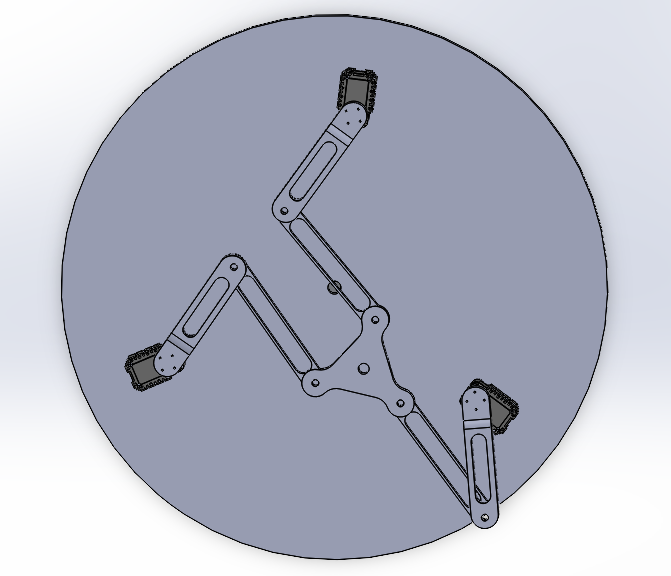
\includegraphics[width=\textwidth]{Figures/singularité parallèle.png}
        \caption{Singularité parallèle (droites parallèles)}
    \end{subfigure}
    \begin{subfigure}[t]{0.48\textwidth}
        \centering
        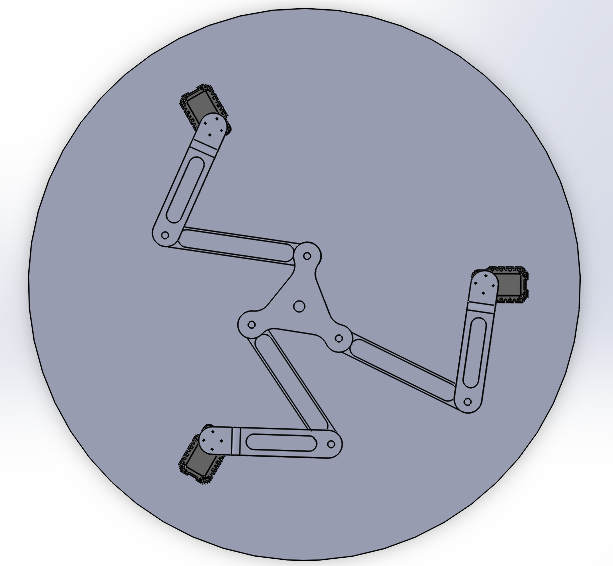
\includegraphics[width=\textwidth]{Figures/singularite parallele concourante.png}
        \caption{Singularité parallèle (droites concourantes)}
    \end{subfigure}
    \caption{Singularite série et parallèles}
    \label{fig:singularity}
\end{figure}

On propose 3 captures d'écrans des 3 différentes singularités sur la figure \ref{fig:singularity}.

\section{Simulation}
Afin de simuler le robot, nous avions accès à des codes en MatLab. Ces codes permettent de calculer le modèle géométrique inverse de façon analytique et numérique, ainsi qu'une fonction permettant de tracer la configuration de l'appareil.

Notre première étape fut de transformer ces codes sous Python afin de les utiliser dans notre simulation. Pour celle-ci, nous avons utilisé la bibliothèque PyGame, qui permet d'afficher des éléments graphiques avec de l'animation. Par simplicité, nous avons créé une classe Robot3RRR pour tous les calculs nécessaire à la simulation.

Notre simulation permet de controller l'effecteur via les touches de notre clavier, mais aussi de dessiner des formes prédéfinis :
\begin{itemize}
    \item un carré
    \item un cercle
    \item un polynôme quelconque
\end{itemize}

Notre méthode \textit{interpolate\_path} prend les points de la figure (par exemple les quatres points du carré) et fait une interpolation entre ces points afin que le robot suive la bonne courbe.
\section{Réalisation}

\section*{Conclusion}
\addcontentsline{toc}{section}{Conclusion}

% \newpage

\newpage
\nocite{*}
\addcontentsline{toc}{section}{Bibliographie} 
\printbibliography
\end{document}